% !TeX spellcheck = en_US
\documentclass[titlepage]{article}
\usepackage{pacco}
	\makeindex
\begin{document}
	\title{Probability theory notes}
	\author{Kotatsu}
	\date{\small TOALDO COL \textbf{CAZZO} CHE DIVENTI ORDINARIO}
	\maketitle
	\pagenumbering{roman}
	\begin{preface}
		This document stems from the fact that I just seem unable to pass the Probability Theory exam for the life of me. I regret with every ounce of my being the fact that I enrolled to the Stochastics and Data Science master degree a year ago. Since dear Professor Toaldo never really thrilled me with his insightful lectures about this delightful topic, I resorted to watch the old lectures by Professor Polito, who at least seems to know the subject and to be determined to explain it.\\
		Unlike many among my esteemed colleagues I have NOT a background in mathematics so there will be a lot of repetitions and possibly mistakes. Do what you want with this information. YES I KNOW that there are the whiteboard registrations of his lectures but if I DECIDED TO DO THIS it was because I couldn't comprehend shit with only those notes.\\
		I'll also try to compile the notes made by Professor Sacerdote, in the vain attempt to overcome the drowsiness that is congenitally entwined with every event that contemplates her uttering any words.\\
		I take much pride in my custom environment and in my packages. If you don't like them I will be very sad. \\
		It is strongly recommended to play Metal Gear Solid, Metal Gear Solid 2 and Metal Gear Solid 3 before reading these notes to fully understand the subject treated.
		
		\vskip1.2cm
		
		\hfill Kotatsu
	\end{preface}
	\clearpage
	\pagenumbering{arabic}
	\tableofcontents
\section{Basics of probability}
We start with the probability triplet: $(\Omega,\mathscr{H},\mathbbm{P})$ 
Here $\Omega$ is the set of sample space, $\mathscr{H}$ is the $\sigma$-algebra built upon $\Omega$ and $\pr$ is the probability measure. Since $\pr$ is a measure, it will take values in $\R$. \\
We are interested in probability measure, which means:
\begin{itemize}
	\item $\pr$ is a \textbf{finite measure} and $\pr(\Omega)=1$;
	\item $\omega \in\Omega$ will be called \textbf{outcomes}.
\end{itemize}
So consider the example of the roll of the die. If we roll it, 
\[\Omega=\underbrace{\left\{1,2,3,4,5,6\right\}}_{\text{outcomes}}\]
And if we considere the elements $A\in\mathscr{H}$ (which will be subsets of $\Omega$) will be called \textbf{events}.\par We want to quantify the possibility that the event $A$ occurs: we want to measure, through $\pr$, the set $A$: from a measure theory point of view, it's only sets in the $\sigma$-algebra. \\The probability measure has the following properties:
\begin{itemize}
	\item $\pr(\Omega)=1,\quad\pr(\emptyset)=0$
	\item \textbf{monotonicity of $\pr$}: take 2 events $H,K\in\mathscr{H}$ such that $H\subset K$. Then $\pr(H)\leqslant\pr(K)$\footnote{note that the notation is loose since we have proper subset on one side and leq on the other side. But this is not much of a problem, since i will kill myself very soon.}.
	\item \textbf{finite additivity}: take $H,K\in\mathscr{H}$ such that $H\cap K=\emptyset$. The $\pr(H\cup K)=\pr(H)+\pr(K)$;
	\item \textbf{countable additivity}: this requires that we consider collection of events. We denote them in this way:
	\[\left(H_n\right)_{n\in\N}\subset\mathscr{H}\] with $\N=\{0,1,2,3,\ldots\}$ and $\N^\star=\{1,2,3,4,\ldots\}$ such that they are disjoint pairwise (except identical pairs). Then
	\[\pr\left(\bigcup_nH_n\right)=\sum_n\pr\left(H_n\right)\]
	\item \textbf{Boole inequality (sub-additivity)}: if we have a collection $\left(H_n\right)_{n\in\N}\subset\mathscr{H}$ (not necessarily disjoint) then $$\pr\left(\bigcup_nH_n\right)\leqslant\sum_n\pr\left(H_n\right)$$ 
	\item \textbf{sequential continuity}: consider the sequence $\left(H_n\right)_{n\in\N}\subset\mathscr{H}$ such that $H_n\nearrow H\in\mathscr{H}$ ($H_n$ is an increasing sequence of numbers that has $H$ as limit) then $\pr(H_n)\nearrow\pr(H)$. Moreover, if $\left(F_n\right)_{n\in\N}\subset\mathscr{H}$ such that $F_n\searrow F\in\mathscr{H}$ then $\pr(F_n)\searrow\pr(F)$. The second property is actually true because $\pr$ is finite (it is not true for infinite measures). 
\end{itemize}
In measure theory we encounter the concept of \textbf{negligible sets}: these are sets of measure zero or non measurable sets included in measure zero sets. In probability theory, sets are \textbf{events}: so we have negligible events (events with probability 0 or non measurable events included in events with probability 0). Analogously, in measure theory a property which holds \textbf{almost everywhere} is allowed not to hold on negligible sets. In probability theory a property which holds \textbf{almost surely} is allowed not to hold on negligible events.
We also have, in measure theory, \textit{measurable functions} that in probability theory are \textbf{random variables}.
Let's have a look back into what the absolute fuck a measurable function is. Also what is an integral? This course deals with distributions, measures and other hellish machinery that servers the sole purpose to confuse you.
\begin{revise}
	\begin{definition}
		Let $(E,\mathscr{E}$ and $(F,\mathscr{F})$ be measurable spaces. A mapping $f:E\mapsto F$ is said to be \enf{measurable} relative to $\mathscr{E}$ and $\mathscr{F}$ if 
		\[f^{-1}(B)\in\mathscr{E}\qquad\every B\in\mathscr{F}.\]
	\end{definition}
	There is an useful property to measurable functions. Take a function $f:E\mapsto F$. In order for $f$ to be measurable relative to $\mathscr{E}$ and $\mathscr{F}$ it is necessary and sufficient that
	\[f^{-1}(B)\in\mathscr{E}\qquad\every B\in\mathscr{F}_0\]
	where $\mathscr{F}_0$ is a collection that generates $\mathscr{F}$, i.e. $\mathscr{F}=\sigma(\F_0)$.
\end{revise}
\subsection{Random variables}
Consider a measurable space $(E,\mathscr{E})$. 
\begin{definition}
	A mapping $X:\Omega\rightarrow E$ is called \enf{random variable taking values in $E$} if $X$ is measurable relative to $\mathscr{H}$ and $\mathscr{E}$.
\end{definition}
What does it mean\footnote{who asked}? The inverse image of the set $A$ through $X$ ($X^{-1}A$) with $A\in \mathscr{E}$ is actually the set of the $\omega$s such that $X(\omega)$ arrives to $A$. So
\[X^{-1}A=\left\{\omega\in\Omega:X(\omega)\in A\right\}=\left\{X\in A\right\}\] so that $X^{-1}A$ is an event for all $A$ in $\mathscr{E}$.
\begin{figure}[H]
	\centering
	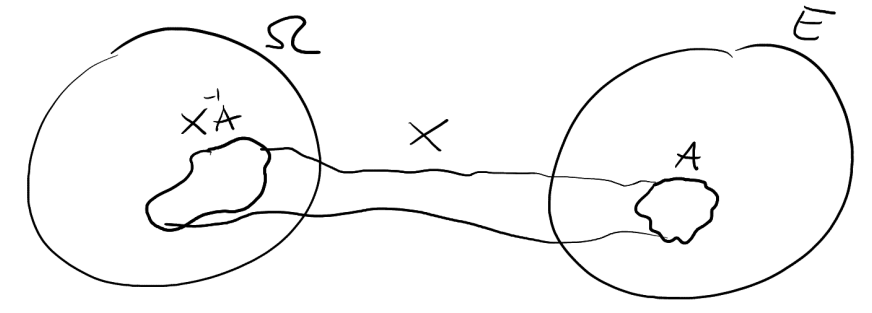
\includegraphics[width=0.8\linewidth]{screenshot001}
	\caption{this is an early reminder of the fact that I will take my own life very soon.}
	\label{fig:screenshot001}
\end{figure}
So if $X^{-1}A$ is measurable by $\pr$ then it is in $\mathscr{H}$: otherwise it is not in $\mathscr{H}$. So \[\pr(X^{-1}A)=\pr\left(\left\{\omega\in\Omega:X(\omega)\in A\right\}\right).\] The message is that I am interested/able to evaluate $\pr$ over the set only if what I am evaluating is indeed an event (which means: it belongs to $\mathscr{H}$\footnote{il lettore più arguto avrà notato che, a questo punto, il dio è ormai irrimediabilmente cane.}). If something is not in $\mathscr{H}$ get it off my fucking face man and kill yourself NOW\footnote{
		
\includegraphics[width=0.05\linewidth]{screenshot002}
}. This is the only restriction for a random variable. $E$ can be whatever we need it to be: a graph, a tree, your mom being absolutely \censor{torn apart} by me. But most of the times, we have $E=\R$ or $E=\R^d$ with respectively $\mathscr{E}=\mathscr{B}\footnote{Borel \sa. You don't know what a Borel \sa\; is? \url{https://en.wikipedia.org/wiki/Borel_set}}(\R)=\mathscr{B}_\R$ and $\mathscr{B}_{\R^d}$.
\begin{remark}
	The simplest random variables are indicator functions of events.
	Example: take $H\in\mathscr{H}$. Define the function
	\begin{align*}
		\indi_H&:\Omega\rightarrow\R\\
		\indi_H(\omega)&=\begin{cases}
			0 &\omega\not\in H\\
			1 &\omega\in H
		\end{cases}
	\end{align*}
\end{remark}
\begin{remark}
	A random variable is said to be \enf{simple} if it takes only finitely many values in $\R^d$.
\end{remark}
\begin{remark}
	A random variable is said to be \enf{discrete} if it takes only countably many values.
\end{remark}
We are now ready to define the concept of \textit{distribution of a random variable}. But first...
\begin{figure}[H]
	\centering
	\begin{tikzpicture}
	\lemmethink[width=4.3cm,position={(-1,-1)},fill=white]{Yeah I don't know about you guys but I have the uncomfortable sensation that we are about to talk about distributions and I won't be able to see a goddamn integral like I am used to do. Can we address this fact please?}
\end{tikzpicture}
\end{figure}
Sure. Let's have a look back to Lebesgue integration.
\begin{tcolorbox}[enhanced jigsaw,sharp corners, drop fuzzy shadow=gray,colback=white,frame style={white},interior style={fill stretch image=lebe},width=\linewidth,height=0.27\linewidth]
\end{tcolorbox}
	\begin{revise}
		Consider a measure space $(E,\mathscr{E},\mu)$. $\E$ can be seen as the collection of all $\E$-measurable functions $f:E\mapsto\overline{\R}$ on $E$ that can be denoted with an abuse of notation\footnote{I am the only one being abused here.} by $f\in\E$ and by $d\in\E_+$ if the functions are positive. Our aim is to define integrals of measurable functions with respect to the measure $\mu$ so that:
		\[\mu f=\mu(f)=\int_E f(x)\mu(\dx)=\int_Ef\dif\mu\]
		which is written as the product of $\mu$ and $f$. It is interesting to note, in the last part of the equation, that the integral reads something like: "integrate $f$ over $E$ with respect to the measure $\mu$". What is this measure?? This is the question. Turns out that the good old Riemann integral is just a particular case of the Lebesgue integral when a certain measure is chosen.\\
		 We consider them as the generalization of vectors and hence the scalar product becomes a sum, which transforms into an integral. We will define the Lebesgue integral in three steps:
		\begin{enumerate}
			\item Simple and positive functions:
			\begin{definition}
			The function $f$ is called a \enf{simple and positive function} if it can be written as $$\sum_{i=1}^{n}a_i\indi_{A_i}$$ where $A_i\in\E$ and $a_i\geq0\in\R$ for $i=1,2,\ldots,n$.
			\end{definition}
			\begin{definition}
				For simple and positive functions, we define the Lebesgue integral as 
				\[\mu f:=\sum_{i=1}^{n}a_i\mu(A_i)\]
			\end{definition}
			\item Positive and measurable functions:
			\begin{theorem}
				Let $f\in\E_+$. Then there exists a sequence of simple and positive functions $f_n$ such that $f_n\nearrow f$.
			\end{theorem}
			Thanks to this theorem, we can well pose the following definition"
			\begin{definition}
				Let $f\in\E_+$. We define
				\[\mu f:=\lim_{n}\mu f_n\]
				where $f_n$ is a sequence of simple and positive functions such that  $f_n\nearrow f$.
			\end{definition}
			\item Recall a general fact for real-valued functions.
			\begin{remark}
				Let $f$ be a real-valued function. Then we can write
				\[f=f^+-f^-\]
				With $f^+:=f\vee0=max\{f,0\}$, called \emph{positive part} and $f^-:=-(f\wedge0)=-min\{f,0\}$, called \emph{negative part}. Both of them are real and positive functions and $f$ is measurable \underline{if and only if} $f^+$ and $f^-$ are real and positive functions.
			\end{remark}
		\end{enumerate}
		We are now ready to define the Lebesgue integral for measurable functions in $\R$. The trick is to separate the positive and the negative part of the function, to treat them as the limit of sequence of simple functions and then lose ourselves in the bliss of measure theory.
		\begin{definition}
			Let $f\in\E$. We define
			\[\mu f:=\mu(f^+)-\mu(f^-)\]
			Provided that \underline{at least} one of the integrals is finite in order to be defined and not incur into indefinite forms like $+\infty$ or $-\infty$.
		\end{definition}
		This definition can be easily converted if $f$ is a complex function: we only have to remember that we can decompose any complex number in its real and imaginary part. Both of them will be measurable real functions.
		\[f=\mathfrak{Re}^+f-\mathfrak{Re}^-f+i(\mathfrak{Im}^+f-\mathfrak{Im}^-f).\]
		From now on we will use this notation for the Lebesgue integral on $(E,\E)$:
		\[\mu f=\int_Ef(x)\mu(\dx)\qquad\text{with }f\in\E\]
		and if we choose $f=\indi_B$ with $B\in\E$. then
		\[\mu f=\mu \indi_B=\int_E\indi_B(x)\mu(\dx)=\indi_B\mu(\dx)=\mu(B).\]\par
		So this last equivalence helps us to understand one thing. \underline{Integrals are a device that needs a measure and a function to work}. In the notation above, $\dx$ has the meaning of an infinitesimal amount of the variable $x$ that is fed into the function $f$. Writing $\mu(\dx)$ means measuring an infinitesimal amount of $x$ using the measure $\mu$.\\
		In Riemann integration, $\dx$ represents an infinitesimal segment of the $x$-axis multiplied by the height of the function at $x$ (which is, of course, $f(x)$) and summed ($\int_{a}^{b}$) with all the other infinitesimal segments of the $x$-axis over the interval $[a,b]$. \\
		Here it's really the same thing with the difference that we multiply the height of the function $f(x)$ by calculating the "weight", or "\underline{measure}" of a smaller and smaller part of the domain that "causes that function to be of that height", according to our method of measure of choice. We do this over the set $E$.\par	
	\end{revise}
	\begin{tcolorbox}[enhanced jigsaw,sharp corners, drop fuzzy shadow=gray,colback=white,frame style={white},interior style={fill stretch image=lebe2},width=\linewidth,height=0.27\linewidth]
	\end{tcolorbox}
The main difference between Riemann and Lebesgue integration is, in a certain way, \textit{what} we are slicing. In the Riemann approach be basically do the following:
\begin{enumerate}
	\item slice the $x$-axis in smaller and smaller slices;
	\item compute $f(x)$;
	\item sum all the cute little rectangles you got.
\end{enumerate}
In the Lebesgue approach we basically \textit{start by choosing different slices of the }range\textit{of the function}, that is the co-domain. These little "slabs" of the range of the functions are nothing else but the "stepped" simple function version of our function:
\begin{figure}[H]
	\centering
	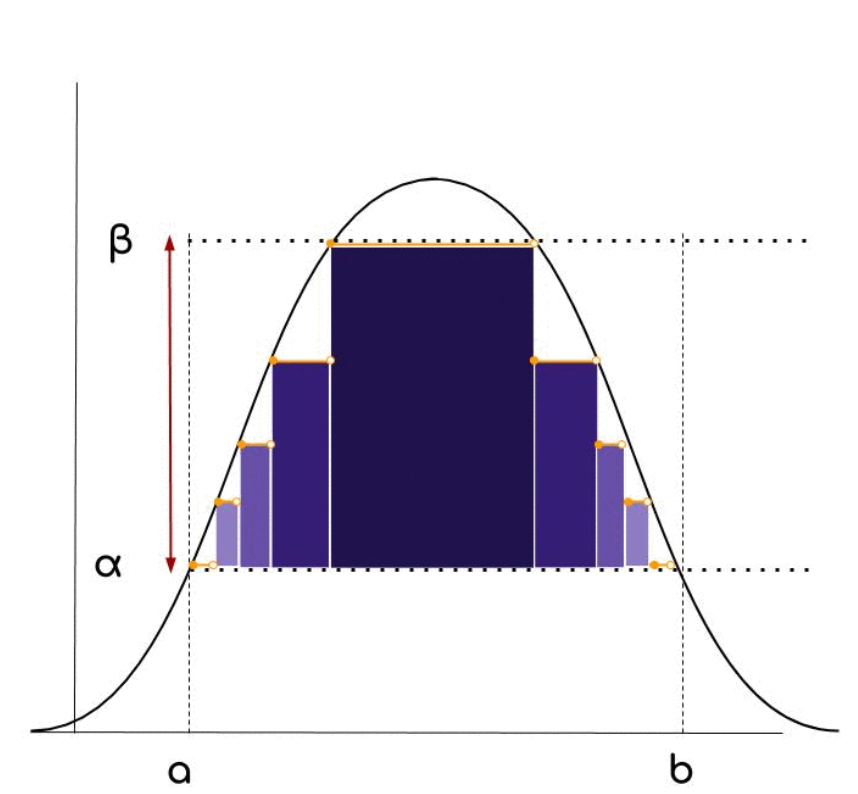
\includegraphics[width=0.46\linewidth]{screenshot004}
	\caption{Imagine the steps getting smaller and smaller...}
	\label{fig:screenshot004}
\end{figure}
Since we are dealing with simple functions, we are effectively approaching the problem from the $y$-axis. This means that since we are choosing slices of height \textit{first} our "slabs" may have different length when it comes to the $x$-axis. Anyway was it really SO DIFFICULT to explain? I don't think so. Fuck you mathematicians.\\
	So... will there ever be a measure and a set for which we will be able to circle back to our definition of Riemann integral? Hmm...\par
\begin{definition}
	\enf{Distribution of a random variable}. Let $X$ be a random variable taking values in $(E,\mathscr{E})$ and let $\mu$ be the image of $\pr$ under $X$, that is,
	\[\mu(A)=\pr(X^{-1}A)=\pr(X\in A)=\pr\circ X^{-1}(A)\footnote{you would know this if you knew fucking measure theory I guess},\;A\in\mathscr{E}.\] Then $\mu$ is a probability measure on $(E,\mathscr{E})$ and it is called \textbf{distribution of X}.
\end{definition}
So we map, by means of $X$, sets belonging to $\mathscr{E}$ into $\mathscr{H}$ and then evaluates this sets by means of the measure $\pr$. This is what we mean when we say that distributions are ultimately built with the probability measure and the random variable. \\
Distribution is itself a measure. To be exact it is a measure that we employ with a function (that in our case is a \rv{}) to form a Lebesgue integral just like we have seen in the revise box above. As we said, integrals are a machine that needs a function and a measure;
 in the case of probability theory these elements are respectively the \emph{random variable} and the \emph{probability distribution}.\\
 Right now we can start to see the light at the end of the tunnel\footnote{This is only the first chapter.} and start to have an intuition for all the ingredients to create this soup called "probability theory". Distributions are NOT cumulative density functions and neither they are probability density functions... They are something that transcends these "specialized" concepts and goes to the heart of how we evaluate (how we weigh; how we \textbf{measure}) a probability in a certain scenario. 
\begin{center}
	 Distributions are probability measures.
\end{center}
\begin{remark}
	You should remember (LOL) that when we want to specify a measure on a $\sigma$-algebra, it's enough to do it on a \textit{$\pi$-system}\footnote{a $\pi$-system is a simpler object than a $\sigma$-algebra: it is simply a collection of sets closed under intersection} generating that $\sigma$ algebra: by means of the monotone class theorem we are then able to extend the measure to the $\sigma$-algebra. \\
	This means that to specity $\mu$ it is enough to specify it on a \textit{$\pi$-system} which generates $\mathscr{E}$. For example, consider $E=\overline{\R}, \mathscr{E}=\mathscr{B}_{\overline{\R}}$. Consider the collection of sets $[-\infty,x],\;x\in\R$ which is of course a $\pi$-system because it is closed under intersection. Moreover, this shit generates the Borel sigma algebra on $\overline{\R}$. \\If we want to define a distribution, that is a measure, it is enough to define it on this $\pi$-system. Imagine that we apply our distribution measure to one set of this $\pi$-system
	\[c(x)\footnote{because it is a function of $x$}=\mu\left([-\infty,x]\right)=\pr(X\leq x),\qquad x\in\R\] by the monotone class theorem. So we have now specified the measure on the $\pi$-system. The part $\pr(X\leq x)$ reminds us of the undergraduate times\footnote{I already wanted to kill myself at that time.}: it is a distribution function! This is what our professor did implicitly to avoid using measure theory\footnote{I have noticed that my life has not benefited in ANY form since I have been introduced to measure theory.}.
\end{remark}
\begin{revise}
	But what is the \textit{monotone class Theorem}? First, we need the definition of \textit{monotone class}:
	\begin{definition}
		A collection of functions $\mathcal{M}$ is called \enf{monotone class} provided that:
		\begin{enumerate}
			\item it includes the constant function 1;
			\item taken $f$ and $g\in\mathcal{M}_b$ (with $\mathcal{M}_b$ being the subcollection of bounded functions in $\mathcal{M}$) and $a,b\in\R$, then $af+bg\in\mathcal{M}$;
			\item if the sequence $(f_n)_{_n}$ is contained in $\mathcal{M}_+$ (with $\mathcal{M}_+$ being the subcollection consisting of positive functions in $\mathcal{M}$) and $f_n\nearrow F$ then $f\in\mathcal{M}$.
		\end{enumerate}
	\end{definition}
	\begin{theorem}
		\enf{Monotone class Theorem}:\\
		Let $\mathcal{M}$ be a monotone class of functions on $E$. Suppose, for some $\pi$-system $\mathcal{C}$ generating $\mathscr{E}$, that $\indi_A\in\mathcal{C}$ for every $A\in\mathcal{C}$. Then $\mathcal{M}$ inclueds all positive $\E$-measurable functions and all bounded $\E$-measurable functions.
	\end{theorem}
\end{revise}
So, turning back to the previous remark: in that case $\E$ consists of the Borel \sa{} on the extended real line ($\B_{\overline{\R}}$); our $\pi$-system is capable of generating the Borel \sa{} (because every Borel set can be constructed with the combination $[-\infty,x]$ for all $x\in\R$\footnote{I know, I know: the fuck is a Borel set? A Borel set is every set that can be formed by the countable union or countable intersection or complementation from any open or closed set. You see that every Borel set you can imagine can be constructed by $[-\infty,x]$.}); we defined the measure $\mu$ on the $\pi$-system $[-\infty,x]$ for all $x\in\R$; the monotone class theorem states that if a class of sets (in this case, the class of sets where $\mu$ is well-defined) contains a $\pi$-system (\checkmark) and is closed under monotone limits (i.e. is a \underline{monotone class}), then it contains the $\sigma$-algebra generated by the $\pi$-system: this means that the class of sets where the distribution $\mu$ is well-defined will include the Borel \sa{} $\B_{\overline{\R}}$. This is kinda cool, I'll have to admit. Unfortunately, I don't really care about this.
\subsection{Functions of random variables}
Consider $X$, a random variable taking values in $(E,\mathscr{E})$ and consider further a measurable space $(F,\mathscr{F})$. Let $f:E\rightarrow F$ be a measurable function relative to $\mathscr{E}$ and $\mathscr{F}$\footnote{This basically means that this bitch won't do anything evil. The whole point of measure theory, $\sigma$ algebras and all other shit is to ensure everything behaves.}. This function should me measurable by means of $\pr$, otherwise we couldn't do anything useful with it. Consider the composition
\[Y=f\circ X\qquad\text{such that}\;Y(\omega)=f\circ X(\omega)=f\big(X(\omega)\big),\;\omega\in\Omega.\]
This composition is a random variable taking values in $(F,\mathscr{F})$ which comes from the fact that measurable functions of measurable functions are still measurable. 
\begin{definition}
	Consider two random variables $X,Y$ taking values in $(E,\mathscr{E})$ and $(F,\mathscr{F})$ respectively. Consider the pair
	\[Z=(X,Y):\Omega\rightarrow E\times F.\]
	Why would we want to call it $Z$? It's because, beside being a random vector, it is in turn a random variable:
	\[Z(\omega)=(X(\omega),Y(\omega)).\]
	Since $E\times F$ is a product space, we should attach it the product $\sigma$-algebra. So $Z$ is a random variable taking values in $E\times F$. 
\end{definition}
Note that the product space $E\times F$ is endowed with the \sa $\mathscr{E}\otimes\mathscr{F}$, that is the product \sa generated by the collection of all possible rectangles between $E$ and $F$. We frequently have to look to special cases like random vectors that must take values in measurable spaces for them to make sense. This measurable space is naturally generated by the product \sa (but it may be generated by other $\sigma$-algebras\footnote{Repeatedly inflicting painful kicks on my gonads.}!).
\begin{definition}
	We call \enf{joint distribution} of $X$ and $Y$ the distribution of $Z$. 
\end{definition}
This is interesting, since we know that this variable has the specific structure of a random vector: we identify the distribution of this vector as the joint distribution of its two coordinates\footnote{it eludes me how anyone could find this interesting. We have to think about the whole vector as being distributed like its components separately}. 
\begin{remark}
	The product \sa{} $\mathscr{E}\otimes\mathscr{F}$ is generated by the $\pi$-system of measurable rectangles.
\end{remark}
On the product space, it is enough to only specify it on this $\pi$-system.\par
Let denote with $\pi$ the joint distribution of $X,y$. It is sufficient to specify
\[\pi(A\times B)=\pr(X\in A, Y\in B)\qquad\every  A\in\mathscr{E},B\in\mathscr{F}.\]
We exploited the measurability of $X$ and $Y$
\begin{definition}
	Given the joint distribution $\pi$, consider sets $A\in\mathscr{E},B\in\mathscr{F}$. Then we call \enf{marginal distribution of $X$}
	\[\pr(X\in A)=\pi(A\times F)\qquad\;\every  A\in\mathscr{E}\]
	and we call \enf{marginal distribution of $Y$}
	\[\pr(Y\in B)=\pi(E\times B)\qquad\;\every  B\in\mathscr{F}.\]
\end{definition}
We call it distribution because it is actually a measure! So we can call it with the notation of measure
	\[\mu(A)=\pr(X\in A)=\pi(A\times F)\qquad\;\every  A\in\mathscr{E}\] and \[\nu(B)=\pr(Y\in B)=\pi(E\times B)\qquad\;\every  B\in\mathscr{F}.\]This actually means that the second coordinate is fixed in being the \underline{whole space} $F$. Think about integrating the second coordinate along the real line when doing marginal distributions... this is the same thing here.\\
Now that we have joint and marginal distributions, what is the next step\footnote{Abandoning myself in the sweet embrace of Death, methinks.}?
\begin{definition}
	Let $X,Y$ be \rv s taking values in $(E,\mathscr{E})$ and $(F,\mathscr{F})$ respectively and let $\mu$ and $\nu$ be their respective distributions. Then $X$ and $Y$ are said to be \enf{independent} if their joint distribution is the product measure formed by their marginals.
	\[\pr(X\in A,Y\in B)=\pr(X\in A)\pr(Y\in B)\qquad\every  A\in \mathscr{E},B\in\mathscr{F}.\]
	This also means that 
	\[\pi=\mu\nu\]
\end{definition}
Here the marginals do not interact with each other. This is true for two random variables but we need\footnote{No.} something more general.
\begin{definition}
Let $(X_1,X_2,\ldots,X_n)$ be a finite collection of random variables. The collection is said to be an \enf{independency} if the distribution of $(X_1,X_2,\ldots,X_n)$ is the product of $\mu_1,\mu_2,\ldots,\mu_n$ where $\mu_i$ is the distribution of $X_i$, for $i=1,\ldots,n$.
\end{definition}
Çinlar is stupid I wish him dead to be frank for this independecy shit. Independecy is not even an english word. What the fuck? Anyway, what about infinite collections?
\begin{definition}
	Let $(X_n)_{_n}$ be an infinite collection of \rv s. It is said to be an \enf{independency} if every finite sub-collection of it is an independecy.
\end{definition}
We now turn to stochastic processes\footnote{Please no.}! But first...
\subsection{Infinite product spaces}
Let $T$ be an arbitrary (countable or uncountable) set. We will think about this set as an "index" set. For each $t\in T$ consider the measurable $(E_t,\mathscr{E}_t)$. So we have a space for each index (plenty of measurable spaces hanging around). Consider a point $x_t$ in $E_t$ for each $t\in T$. The collection\footnote{We could consider it a function of $t$ but that wouldn't be exactly correct since each $t$ has a different measurable space. We may have the same space but it's not true in general... I am thrilled to say the least.} $(x_t)_{_{t\in T}}$. If  $(E_t,\mathscr{E}_t)=(E,\mathscr{E})$ then $(x_t)_{_{t\in T}}$ is actually a function of $T$ taking values on $(E,\mathscr{E})$. \\
The set $F$ of all possible functions $x=(x_t)_{_{t\in T}}$ is called the \enf{product space} $\left((E_t\mathscr{E}_t)\right)_{_{t\in T}}$.\\ This is the natural generalization of what we do when we construct product spaces, albeit with a different notation. Usually $F$ is denoted by $X_{t\in T}E_t$. But we know we also need a \sa...\\
A \enf{rectange} in $F$ is a subset of the form
\[\{x\in F:x_t\in A_t \;\every t\in T\}\]
Where $A_t$ differs from $E_t$ for only a finite number of $t$. So I want to consider subsets of $F$ (the space of functions) of the form above. I want only the functions $x$ in $F$ such that each coordinate belongs to $A_t$, a subset of $E_t$ for each $t\in T$. It seems that we have a restriction on all the coordinates... But this may bring to problems when we have an uncountable number of coordinates and therefore an uncountable number of restrictions. But we can says that if $A_t=E_t$ (the whole space) we don't apply any restriction. So in this case  $X_t$ belongs to $E_t$ so we can choose whatever $X_t$ we like. So only a finite number of coordinates are restricted while the other infinite ones are free to vary\footnote{
\includegraphics[width=0.08\linewidth]{screenshot003}$\rightarrow$ my honest reaction.
}. \par
The \sa{} generated by the collection of all measurable rectangles is denoted by 
\[\bigotimes_{t\in T}\mathscr{E}_t.\]
This is the product \sa{} in any infinite-dimensional space. So, the (natural) resulting measurable space in the end will be
\[\bigtimes_{t\in T}E_t,\bigotimes_{t\in T}\mathscr{E}_t.\] This is not in contrast with what we already know for finite product space, since these already have a finite number of restrictions. So this concept of rectangle, which can be a bit different from the one regarding the famous and well-tested geometrical shape\footnote{Oh thank god someone finally said it. I was starting to get scared.}, is not restricted on all the coordinates (like the shape\footnote{I swear to god.}) but only on a finite number of them. \\
We also have an alternative notation for this measurable space!
\[\bigotimes_{t\in T}(E_t,\mathscr{E}_t).\]
In the case that $(E_t,\mathscr{E}_t)=(E,\mathscr{E})\;\every t\in T$ the product space is denoted by
\[(E,\mathscr{E})^T\] or 
\[(E^T,\mathscr{E}^T)\]
These are not real powers but it's just notation... Anyway these are all different notations to indicate the infinite product space with the product \sa{} built upon the $\pi$-system which is the collection of all possible rectangle defined in the way we saw above\footnote{NO I WON'T USE LABELS AND NUMBERED EQUATIONS.}.
\subsection{Stochastic processes}
\begin{definition}
	Let $(E,\mathscr{E})$ be a measurable space and consider an index set $T$ (as before, an arbitrary set countable or uncountable).\\
	Let also $X_t$ be a \rv{} taking values in $(E,\mathscr{E})$. Then the collection of those random variables $(X_t)_{_{t\in T}}$ is called a \enf{stochastic process} with state space $(E,\mathscr{E})$ and parameter set $T$.
\end{definition}
Note that there is no mention about time here. Just think about the index set, which indexes the stochastic process. If we interpret $T$ as time then we have the most common interpretation of stochastic processes. But it could also be space (imagine $\R^2$) or your mom being \censor{fucked hard}. Anyway the most natural interpretation is time.\par
Now take a $\omega\in\Omega$ and evaluate all these \rv s on the same $\omega$. What we get is
\[t\mapsto X_t(\omega)\]
which is a function from $T$ to $(E,\mathscr{E})$. So if we see it as a function of $t$ for each $\omega$ we get a function which is an element of $E^T$. So what is a stochastic process, to sum it up? It's just a random variable taking values in the infinite product space $E^T$. That's why it is a problematic object: it's because mathematicians deserve to experience the sadness and evil they unleashed upon the world. Ever noticed how similar the words "measurable" and "miserable" are? I didn't think so. 
\begin{figure}
	\centering
	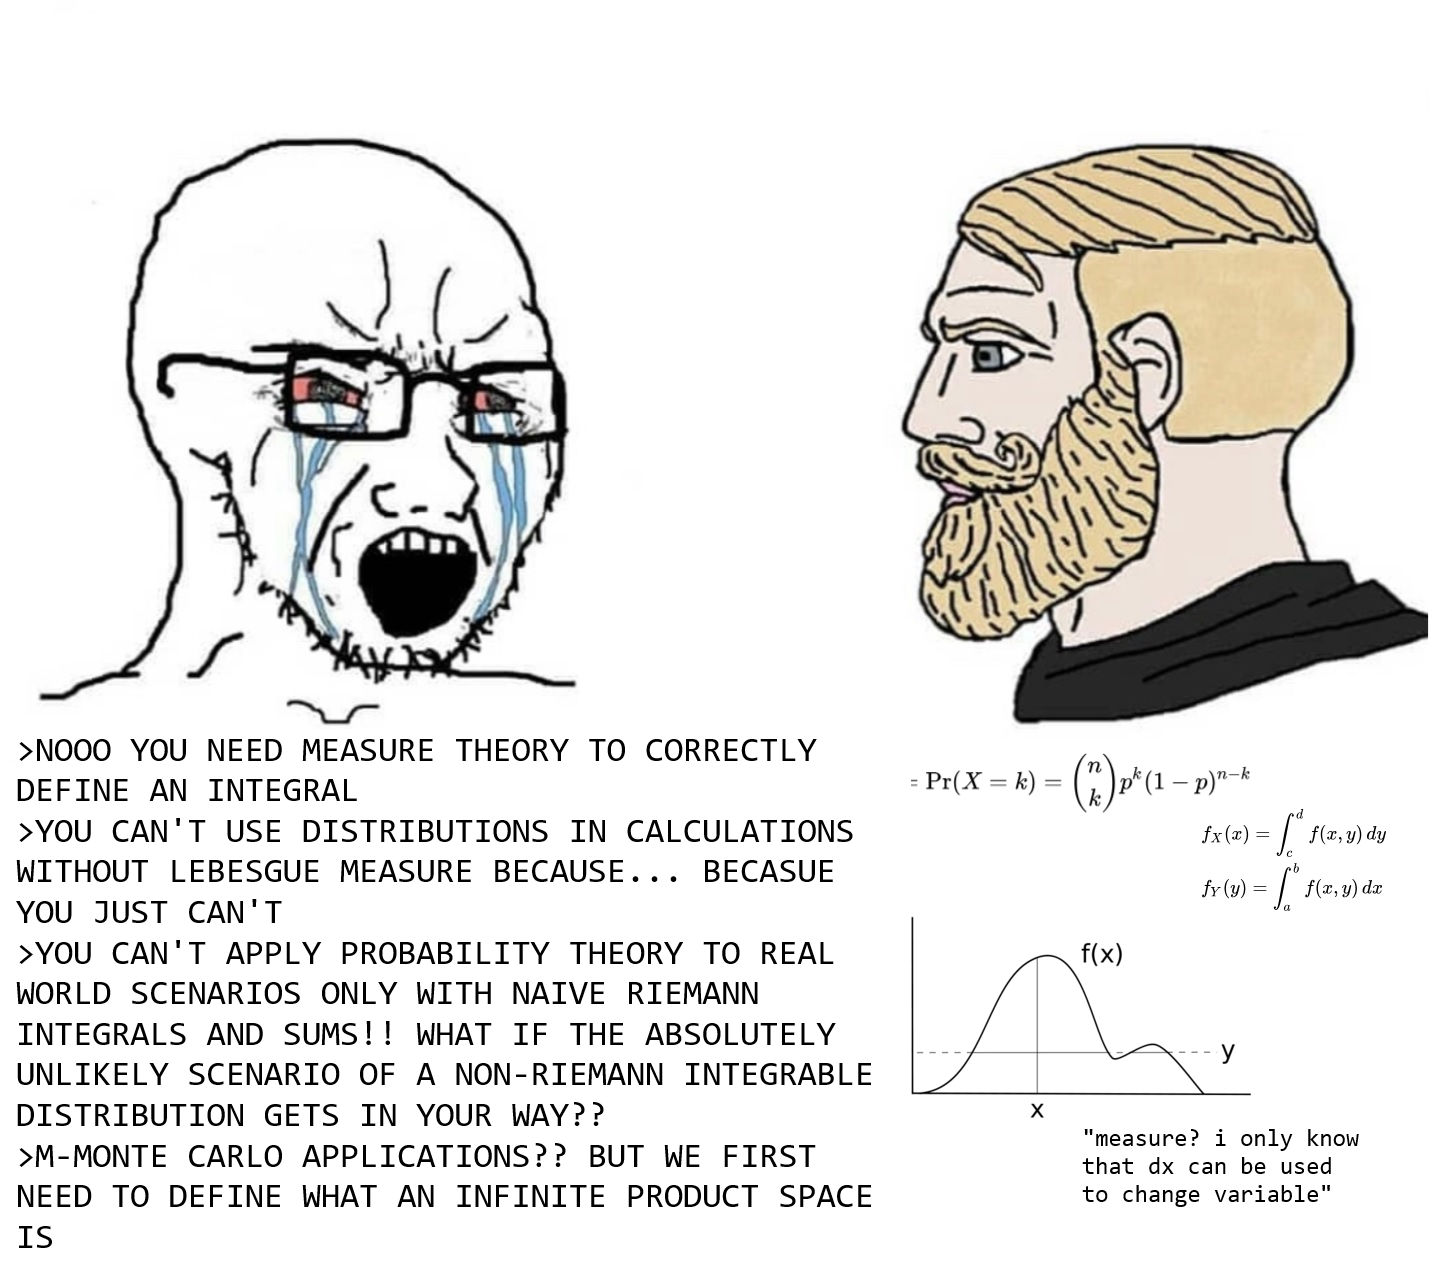
\includegraphics[width=0.6\linewidth]{ILMEMINO}
	\caption{I'm sorry but here you're the soyjack and I'm the chad.}
	\label{fig:ilmemino}
\end{figure}
Yeah technically more structure helps us modeling real phenomena more accurately but who the FUCK cares. 
\subsection{Example of random variables}
Consider some examples of simple random variables:
\begin{example}
	\enf{Poisson \rv s.}\\
	This \rv{} takes vales in $\N$ (it's a one dimensional \rv{}). We consider the power set of $\N$\footnote{Subset of all subsets of $\N$.}. We know that power sets \textit{are} \sa s that we can use (but we could encounter some trouble with uncountable elements, for which we would need smaller \sa s\footnote{No one really cares, not even Federico Polito.}).\\
	What is the distribution of this \rv{}?
	\begin{align*}
	\mu(A)=\pr(X\in A)&=\sum_{n\in A}\pr(X=n)\qquad A\subset\N\\
	\text{with } \pr(X=n)&=e^{-c}\frac{c^n}{n!}, \;n\in\N,\;c>0.
	\end{align*}
	So imagine we have this kind of random variable. We consider a subset of the natural number and we want to evaluate the measure of this subset that we chose. We know that we define the \rv{} by defining the distribution. For each $n$ we get a number $e^{-c}\frac{c^n}{n!}$. Another interesting implication is that \[\sum_{n\in A}\pr(X=n)=\sum_{n\in\N}\delta_n(A)\pr(X=n)\] where $\delta_n(A)$ is the \enf{Dirac measure} sitting at $n$. So, $n$ is a parameter and 
	\[\delta_n(A)=\begin{cases}
		1 &n\in A\\
		0 &n\not\in A
	\end{cases}.\] The Dirac measure is similar to the indicator function (they behave basically in the same way) but the difference is that this one is a \textit{measure} and the latter is a \textit{function}. The Dirac measure has $n$ as a parameter, while the indicator function has the set as a parameter ($\indi_A(n)$).
\end{example}
\begin{example}
	\enf{Exponential \rv{}}\\
	This random variable is again one-dimensional but this time this random variable is \textit{absolutely continuous}. What does it mean? It actually means that the variable is absolutely continuous with respect to the Lebesgue measure\footnote{'tacci tua.}. This is evident when we write down the distribution.\\
	Consider a \rv{} taking values in $\R_+$ and further consider $\mathscr{B}_{\R_+}$. We have
	\[\mu(\dif x)=\underbracket{\dif x}_{\mathclap{Leb(\dif x)}}ce^{-cx},\qquad c>0,\;x\in\R_+.\]
	Ok no wait hold your fucking horses, cowboy. Why did we write $\dif x$ instead of just $x$? Also weren't densities, like, a fucking measure of some set in the form of $\mu(A)$? I like the fact that these densities resemble more closely the probability density function I was taught to work with during my sad Economics degree but there are many many things that creep me out. \par
	We have an answer for this, but we need to do a bit of backtracking.
\end{example}
	\begin{revise}
		First of all: what does "absolutely continuous" \textit{even means}?
		\begin{definition}
			let $\mu$ and $\nu$ be measures on a measurable space $(E,\mathscr{E})$. Then, measure $\nu$ is said to be absolutely continuous with respect to measure $\mu$ if, for every set $A\in\E$,
			\[\mu(A)=0\implies\nu(A)=0.\]
		\end{definition}
		Huh. That was pretty simple. Well, turns out we can exploit this fact to "switch" between different measures inside of integrals...
		\begin{theorem}
			\emph{Radon-Nikodyn Theorem}.
			Suppose that measure $\mu$ is $\sigma$-finite and measure $\nu$ is absolutely continuous with respect to $\mu$. Then there exists a positive $\E$-measurable function $p$ such that 
			\[\int_E\nu(\dx)f(x)=\int_E\mu(\dx)p(x)f(x)\qquad f\in\E_+.\]
			If we use the alternative notation:
			\[\int_Ef\dif\nu =\int_Ep f\dif\mu \qquad f\in\E_+.\]
			Moreover, $p$ is unique up to equivalence: if the equation above holds for another $\hat{p}\in\E_+$ then $\hat{p}(x)=p(x)$ for $\mu$-almost every\footnote{This means that all the setes where this condition doesn't hold are neglegible when weighted with measure $\mu$.} $x\in\E_+$. This is an if and only if statement!\par
			Also, $p$ is called the \emph{Radon-Nikodyn derivative} of $\nu$ with respect to $\mu$:
			\[\frac{\nu(\dx)}{\mu(dx)}=\frac{\dif\nu}{\dif\mu}=p.\]
		\end{theorem}
		With all this alternative notation this thing honestly feels like trying to understand the Metal Gear Solid plot, where identical characters named Snake keep cloning each other and being triple crossed by everyone until you finally understand that the storyline never made sense in the first place and that Hideo Kojima writes his games like a fucking fanfiction.
	\end{revise}
	Now everything should make more sense\footnote{Enviable optimism.}. If we know that a given \rv{} (say, the exponential random variable) has a distribution $\mu(\dx)$ then we will be able to transform this in a distribution of the form $\text{Lebesgue measure}\cdot p(x)$ (we can lose $f$ if $f$ is constant).
	In this formulation	$\dif x$ stands for the Lebesgue measure and the second part of the equation ($ce^{-cx}$) is the $p(x)$, called \emph{density function}. We can do this because we can see from the formula that this distribution, or measure, is indeed absolutely continuous with respect to the Lebesgue measure since we can express it in the form stated by the Radon-Nikodyn theorem.
	 So $p(x)=ce^{-cx},\;x\in\R_+$ is the density relative to $\mu$. This should serve us as a demonstration that if we define the \rv{} we get the distribution/measure (remember! distributions are measures!) and vice versa.

It is interesting\footnote{Debatable claim.} to see that also discrete random variable turns out to be absolutely continuous... But not with respect to the Lebesgue measure. To exact, discrete \rv s are absolutely continuous with respect to the \textit{counting} measure. And here's why to do all this shit we need the Lebesgue integral: by changing the measure we are using to compute the integral, we can use just one object (the probability distribution) to treat both discrete (using a counting measure, which gives us the cumulative distribution function in the form of a sum) and continuous \rv s (using the Lebesgue measure, which gives us the cumulative distribution function in the form of a Riemann integral.)

\vspace{0.5cm}
\begin{figure}[H]
\hspace{1.5cm}
\begin{tikzpicture}
	\calloutquote[width=5cm,position={(-1,-1)},fill=DodgerBlue4,rounded corners]{\color{white}So you know what a Lebesgue measure is, right?}
\end{tikzpicture} 
\begin{flushright}
	\begin{tikzpicture}
		\calloutquote[width=4cm,position={(1,-1)},fill=Turquoise4!30,rounded corners]{Of course not! Is that a bad thing?}
	\end{tikzpicture}\hspace*{2.5cm}
\end{flushright}
\hspace{2cm}
\begin{tikzpicture}
	\calloutquote[width=3cm,position={(-1,-1)},fill=DodgerBlue4,rounded corners]{\color{white}You were adopted}
\end{tikzpicture}
\caption{Actual conversation happened between me and Professor Lods.}
\end{figure}
So we're due for a little refresh on what the hell a Lebesgue measure is. I'm sorry\footnote{Not really. I mean, I'm sorry for the fact that they \textit{are} mathematicians but that's where my compassion starts and ends.} for our mathematician friends but I need this to be written loud and clear. This is from Professor Lods' Lecture notes from the pre-course in Measure Theory, with the hope that one day I'll be skilled like he is with \LaTeX{} typesetting.
\begin{revise}
Let's have a quick refresh about the Lebesgue measure over the measurable space $(\R,\mathscr{B}_{\R})$. Let $S=\R$. First of all, what is an algebra?
\begin{definition}
	A collection $\Sigma_0$ of subsets of $S$ is called an algebra on $S$ if:
	\begin{itemize}
		\item $S\in\Sigma_0$;
		\item if $A\in\Sigma_0$ then $A^c\in\Sigma_0$ where $A^c=S\setminus A$ is the complementary of $A$;
		\item if $A,B\in\Sigma_0$ then $A\cup B\in\Sigma_0$.
	\end{itemize}
\end{definition}
We also need the concept of pre-measure, which is basically a measure but defined on an algebra (instead of a \sa{}):
\begin{definition}
	Let $\Sigma_0$ be an algebra on $S$ (not necessarily a \sa{}. A mapping $\ell:\Sigma_0\mapsto[0,\infty]$ is said to be a \enf{pre-measure} on $\Sigma_0$ if $\ell(\emptyset)=0$ and for any pairwise disjoints $\{A_n\}_{_n}\subset\Sigma_0$ with $\bigcup_nA_n\in\Sigma_0$ it holds:
	\[\ell\left(\bigcup_{n=1}^\infty A_n\right)=\sum_{n=1}^{\infty}\ell{A_n}.  \] 
	Moreover, a pre-measure $\ell$ is said to be $\sigma$-finite on $\Sigma_0$ if there exists a sequence $\{A_n\}_{_n}\subset\Sigma_0$ with $\bigcup_nA_n\in\Sigma_0$ and $\ell(A_n)<\infty$ for any $n\in\N$.
\end{definition}
We can immediately see that $\bigcup_nA_n\in\Sigma_0$ is an additional assumption: in \sa s this assumption is always met. So if $\Sigma_0$ is a \sa{} any measure on $\Sigma_0$ is a pre-measure. \\
We also need one more thing: the \enf{Caratheodory's extension Theorem}.
\begin{theorem}
	\enf{Charatheodory's extension Theorem}: Let $S$ be a given set and let $\Sigma_0$ be an algebra on $S$ and $\Sigma=\sigma(\Sigma_0)$. If $\ell:\Sigma_0\mapsto[0,\infty]$ is a pre-measure on $(S,\Sigma_0)$ then there exists a measure $\mu$ on $(S,\Sigma)$ such that
	\[ \mu(A)=\ell(A)\qquad \every A \in \Sigma_0. \]
	Moreover, if $\ell$ is a $\sigma$-finite pre-measure on $\Sigma_0$, then such a measure $\mu$ on $(S,\Sigma)$ is unique and $\sigma$-finite.
\end{theorem}Apparently this is one of the principal results in measure theory since it allows to construct measures well-adapted to practical situations: once such measures are constructed, Caratheodory's theorem can go fuck itself off. But the most important question is: why do we care about these total nerds?
Because we can now define
\[\mathcal{C}_0=\{[a,b):-\infty\leq a\leq b\leq\infty\in\R\}\]
and let
\[ \Sigma_0=\left\{\bigcup_{j=1}^N I-J:I_j\in\mathcal{C}_0\;\every j,I_i\cap I_j=\emptyset\text{ if }i\neq j,N\in\N \right\} \]
We can prove without major difficulty that $\Sigma_0$ is an algebra on $\R$. Let's define a pre-measure on $\Sigma_0$ by setting:
\begin{itemize}
	\item $\ell([a,b))=b-a$ for any $b\geq a$;
	\item $\ell((-\infty,b))=\ell((a,\infty))=\ell(\R)=+\infty$;
	\item $\ell\left(\bigcup_{j=1}^N I_j\right)=\sum_{j=1}^{N}\ell(I_j)$ if $\{I_j\}_{_{j=1,\ldots,N}}\subset\mathcal{C}_0$ are pairwise disjoints.
\end{itemize}
It can be checked that this newly defined measure is $\sigma$-finite
Remember that $\sigma(\Sigma_0)=\sigma(\mathcal{C}_0)=\mathscr{B}_\R$, which is the Borel \sa{}. 
Consider, additionally, the result of the Charatheodory's extension Theorem. By stitching all of these amenities together we get:
\begin{theorem}
	There exists a unique measure  on $(\R,\mathscr{B}(\R))$ that we denote $\lambda$ (or $\mathfrak{m}$) and such that
	\[\lambda([a,b))=b-a\qquad\every a<b.\]
	We call this measure the \enf{Lebesgue measure} on $(\R,\mathscr{B}(\R))$.
\end{theorem}
\begin{flushright}
	\begin{tikzpicture}
		\calloutquote[width=6cm,position={(1,-1)},fill=white,rounded corners]{So we just learnt how to FIND A FUCKING INTERVAL ON THE REAL LINE?}
	\end{tikzpicture}\hspace*{1.5cm}
\end{flushright}
\hspace{2cm}
\begin{tikzpicture}
	\calloutquote[width=7cm,position={(-1,-1)},fill=DodgerBlue4,rounded corners]{\color{white}Look, I know that can be seen as useless formalism. And indeed it is! We just formalized the notion of \textit{length}. If we take it to 2-dimensional spaces we end up with the notion of area, in 3-dimensional spaces is the notion of volume... and so on.}
\end{tikzpicture}
\begin{flushright}
	\begin{tikzpicture}
		\calloutquote[width=6cm,position={(1,-1)},fill=white,rounded corners]{Huh. This makes sense. So this is the notion of length when everything, including the real line, is a set. Kinda seems like the solution to a problem we ourselves created...}
	\end{tikzpicture}\hspace*{1.5cm}
\end{flushright}
\hspace{2cm}
\begin{tikzpicture}
	\calloutquote[width=4cm,position={(-1,-1)},fill=DodgerBlue4,rounded corners]{\begin{center}
			
\includegraphics[width=0.5\linewidth]{lool}
	\end{center}}
\end{tikzpicture}
\begin{remark}
	We can define in the same way the Lebesgue measure on $(I, \mathscr{B}_I)$ for all $I\subset\R$.
\end{remark}
\begin{remark}
	The measure space $(\R,\mathscr{B}_\R,\lambda)$ is $\sigma$-finite since $([-n,n))_n\nearrow\R$ but is not finite since
	\[ \lambda(\R)=\lim_{n}\lambda([-n,n))=\lim_{n}2n=\infty\]
\end{remark}
\end{revise}
Yeah, that mysterious measure I was talking about before to connect Riemann and Lebesgue integration was the Lebesgue measure. We often just write $\dx$ to express the Lebesgue measure (which is what we did on example 1.2 about the exponential random variable), but the meaning is always the same, with a striking similarity to the concept of Riemann integration: take the Lebesgue measure of a smaller and smaller element of our $\B_{\overline{\R}}$ set, use it to "weight" (read: multiply) the value of the function for that element and then  sum it all up together. What we end up with is basically a serie of simple functions that slice "horizontally" the co-domain of the function. Keep reducing the size and you end up with the Lebesgue integral. Of course, when the measure is the Lebesgue measure, the Riemann and the Lebesgue integral have a really similar interpretation.\par
Back to our topic: the exponential \rv{} is absolutely continuous with respect to the Lebesgue measure.  
It is interesting to see that also discrete \rv s turn out to be absolutely continuous: the difference is that they are not absolutely continuous to the Lebesgue measure, but the \textit{counting} measure. At the undergrad level we are used to say that a \rv{} is either discrete or absolutely continuous, buy this was ultimately a lie\footnote{Measure theory turns truths into lies. Truly a demonic machinery.}.
\begin{example}
	\enf{Gamma distribution}\footnote{She factorials on my $\gamma$ 'till I $\beta$.}:
	Consider a \rv{} taking values in $\R_+$ and consider as a \sa{} the Borel \sa{} $\mathscr{B}_{\R_+}$. The distribution of the Gamma \rv{} is the following:
	\[\mu(\dif x)=\dif x\frac{c^ax^{a-1}e^{-cx}}{\Gamma(a)},\qquad
	\text{with }
	\begin{array}{l}
		a>0,\\
		c>0,\\
		x\in\R_+
	\end{array}.\]
	Here $\Gamma(a)$ is the \textit{Gamma function:}
	\[
	\Gamma(a)=\int_{0}^{+\infty}e^{-x}x^{a-1}\dx.
	\]
	The Gamma function is one of the most famous special functions that comes up almost everywhere. This definition of Gamma function is valid just for positive values and can be seen as a \textit{Laplace transform}\footnote{$\mathcal{L}\{f\}(s)=\int_{0}^{+\infty}f(t)e^{st}\dif t$ where s is a complex number $s=a+ib$.} or as a \textit{Mellin transform}\footnote{$\mathcal{M}[f;s]\equiv F(s)=\int_{0}^{+\infty}f(t)t^{s-1}\dt$ where $s=a+ib$.}.
	The first parameter $a$ is called \textit{shape parameter}; the parameter $c$ is called \textit{scale parameter}. This distribution is also continuous with respect to the Lebesgue measure. \par
	We have some special cases of the Gamma distribution but Federico Polito doesn't really care about. Just know that the $\chi^2$ distribution is a special case of the Gamma \rv{}.
\end{example}
\begin{example}
	This is a certified hood classic: \emph{Gaussian distribution}.\\
	Consider a \rv{} takinv values in $\R$. Of course we consider $\B_{\overline{\R}}$ and the distribution is (notice how also this one is absolutely continuous with respect to the Lebesgue measure):
	\[\mu(\dx)=\dx\cdot\underbracket{\frac{1}{\sqrt{2\pi b}}e^{-\frac{(x-1)}{2b}}}_{\mathclap{p(x)}},\qquad \begin{array}{l}
	a\in\R,\\
	b>0\in\R,\\
	x\in\R_+
	\end{array}.\]
	Of course, $a$ is called the \textit{mean} of the distribution and $b$ is called the \textit{variance}.
\end{example}
\begin{example}
	This is a random variable that stems from two independent random variables having Gamma distribution. Consider $\gamma_a$ (distribution of a Gamma \rv{} with parameters $a$ and $c=1$) and $\gamma_b$ (distribution of a Gamma \rv{} with parameters $b$ and $c=1$). So, two gammas with different shape parameter. \\
	Let $X\sim\gamma_a$ and $Y\sim\gamma_b$. Moreover, let them be independent. This is a random vector $(X,Y)$ with two components... What is its distribution?
	\[\pi(\dx,\dy)=\underbracket{\gamma_a(\dx)\cdot\gamma_b(\dy)}_{\mathclap{\text{because of independency}}}=\dx\dy\frac{e^{-x}x^{a-1}}{\Gamma(a)}\cdot\frac{e^{-y}y^{b-1}}{\Gamma(b)}.\]
	So it's easy to build joint distributions when the \rv s are independent\footnote{Well no shit. Even I can multiply two numbers}.
\end{example}
\begin{example}
	\emph{Gaussian \rv{} with exponential variance}.\\
	Here the variance is random and is distributed exponentially\footnote{because humans should never have the hubris to meddle with the horrorific world of random necessities that the Gods have laid before us.}. Consider a \rv{} $X$ taking values in $\R_+$ and a \rv{} $Y$ taking values in $\R$.\\
	Here we are again in presence of a random vector. The distribution is the following:
	\[\pi(\dx,\dy)=\dx\dy\cdot ce^{-cx}\frac{1}{\sqrt{2\pi x}}e^{-\frac{y^2}{2x}}\qquad \begin{array}{l}
		x\in\R_+,\\
		y\in\R
	\end{array}. \]
	\begin{remark}
		$\pi$ in this case has a special form: it has the form 
		\[\pi(\dx,\dy)=\mu(\dx)K(x,\dy).\]
		In particular, here $\color{Cyan4}\mu(\dx)$ is 
		\[\color{Cyan4}\dx\color{black}\dy\cdot\color{Cyan4} ce^{-cx}\color{black}\frac{1}{\sqrt{2\pi x}}e^{-\frac{y^2}{2x}},\]
		which is a docile exponential function, and $\color{Magenta4}K(x,\dy)$ is
		\[\color{black}\dx\color{Magenta4}\dy\cdot\color{black} ce^{-cx}\color{Magenta4}\frac{1}{\sqrt{2\pi x}}e^{-\frac{y^2}{2x}}.\]
		In this case $K(x,\dy)$ cannot be the distribution fo $Y$, because it has some $x$ in it. So this distribution is not simply the product of marginal distribution. But let's take a closer look to the form $\mu(\dx)K(x,\dy)$. $\mu(\dx)$ is certainly a measure, but what about $K(x,\dy)$? \par
	\end{remark}
\end{example}
\section{Transition kernels}
Turns out that $K(x,\dy)$, depending on $x$, is connected to the other measure $\mu(\dx)$. \\
The object $K(x,\dy)$ is called \emph{transition kernel}\footnote{Kernel? Colonel? I thought we were over with the Metal Gear Solid jokes.} and it's very important. Not that here 
$K(x,\dy)$ has the form 	
\[B\mapsto K(x,B)\]
It should be seen as a set function. Why? Just look back to $\pi(\dx,\dy)$. It is in differential form, but if we integrate the joint distribution against one set in the product space we get $\pi$ evaluated on that subset of the product function (it is a measure... measures are always set functions). So also $\mu(\dx)K(x,\dy)$ should be a set function. $\mu(\dx)$ is of course a set function (it is a measure...\footnote{All this passive-aggressiveness for what?}) and so should be $K(x,\dy)$. The presence of $x$ in $K(x,\dy)$ is what "links" the $X$ coordinate with the $Y$ coordinate of the random vector.
The Gamma example was about two independent random variables: here it is impossible to obtain the product of measures. Transition kernels are incredibly important because they are ultimately connected with the \textit{structure of dependency} between random variables: that's why this course is going to bust our ball into the oblivion about them\footnote{Professor Polito jokes that every year people complain about the abstractness of kernels and laughs about it. I'm happy that his sense of humor has been left untouched by my slightly scathing EDUMETER review of this course.}.
\begin{figure}[H]
	\centering
	
\includegraphics[width=0.57\linewidth]{codec}
	\caption[Caption for LOF]{Yeah, no more Metal Gear Solid jokes after this one. I promise\protect\footnotemark.}
	\label{fig:codec}
\end{figure}
\footnotetext{This is not, in fact, the last Metal Gear Solid joke.}
Remember in the undergraduate courses: when there was dependence we usually expressed it with the \textit{conditional probability}. \\
Transition kernels let us manage random vectors that are not trivial and that have a dependence relationship with other random vectors. \\
Think about the previous example: the marginal distribution $\nu$ of $Y$ has the form \begin{align*}
	\nu(B)&=\pi(\R_+\times B)=\int_{\R_+}\mu(\dx)K(x,B),\qquad B\in\B_{\overline{\R}}\\
	&=\int_{\R_+\times B}\pi(\dx,\dy)=\int_{\R_+\times B}\dx\dy\cdot ce^{-cx}\frac{1}{\sqrt{2\pi x}}e^{-\frac{y^2}{2x}}\\
	&=\int_B \dy\; n(y),\qquad\text{where }n(y)=\int_{0}^{\infty}\dx \cdot ce^{-cx}\frac{1}{\sqrt{2\pi x}}e^{-\frac{y^2}{2x}}.
\end{align*}
So we have that the marginal distribution $\nu(B)$ is written as $\int_B \dy\;n(y)$ and is therefore absolutely continuous with respect to the Lebesgue measure. We could actually solve this integral ($n(y)$ is a closed form called \textit{two-sided exponent}). So we now have the marginal of $Y$ and the marginal of $X$ and we immediately realize that if we multiply the two densities we do not obtain the joint density (because they are dependent\footnote{OK I GET IT.}).\par
So we are now ready to define the concept of transition kernel.
\begin{definition}
	Let $(E,\E)$ and $(F,\F)$ be measurable spaces. Let $K$ be a mapping from $E\times\F$ into $\overline{\R}_+$. Then $K$ is called \emph{transition kernel} from space $(E,\E)$ into space $(F,\F)$ if:
	\begin{itemize}
		\item the mapping $x\mapsto K(x,B)$ is $\E$-measurable $\every B\in\F$;
		\item the mapping $B\mapsto K(x,B)$ (the second mapping of the kernel, the one regarding the set) is a measure $\every x\in E$.
	\end{itemize}
\end{definition}
We can consider the transition kernel a hybrid object: if we look at it with respect to the first variable it is a \textit{measurable function}, if we look at it with respect to the second variable it is a \textit{measure}.
\begin{example}
	Take $\nu$, a finite measure on $(F,\F)$ and take $k$, a positive function on $(E\times F)$ which is measurable with respect to $\E\otimes\F$, the product \sa{}. Then, we integrate
	\[\int_B\nu(\dy)k(x,y)\qquad\begin{array}{l}
		B\in\F\\
		x\in E
	\end{array}\]
	We see how this object depends on $x$ and on the choice of $B$ (a function of $x$ and $B$...). It defines a transition kernel
	\[K(x,B)=\int_B\nu(\dy)k(x,y)\qquad\begin{array}{l}
		B\in\F\\
		x\in E
	\end{array}\]
	from $(E,\E)$ into $(F,|F)$.
\end{example}
\begin{theorem}
	This theorem tells us what we can do with a kernel. Let $K$ be a transition kernel from $(E,\E)$ into $(F,\F)$. Then, 
	\begin{enumerate}[\circnum]
		\item we have $$\int_F K(k,\dy)f(y)\qquad \text{ with } x\in E,\;f\in\F_+.$$ This operation defines a function $Kf\in\E_+\;\every f\in\F_+$.
		
			\begin{notation}
			The notation $f\in\F_+$ in Çinlar is either the \sa{} $\F$ or the set of functions measurable with respect to the \sa{} $\F$. Another one of the many ways Çinlar chooses to sadden my day. But my revenge is on the way.
		\end{notation}
		 First of all we integrate the kernel with respect to the second variable (which basically means we use it as a measure on $F$). The integrand is $F$ and since this function is a measure with respect to the second variable I can integrate $\F_+$-measurable functions. Remember that $\mu f=\mu(f)=\int_E f(x)\mu(\dx)=\int_Ef\dif\mu$. \\
		The integration over $F$ "takes out" one part of the kernel from the equation (the measure part) so that we can write: \[
	Kf(x)=\int_F K(k,\dy)f(y);
	\]
	\item we want to use the kernel with respect to the first variable (obtaining a $\E$-measurable function), so we integrate 
	\[
	\int_E \mu(\dx)K(x,B)
	\]
	Remember that we must integrate the kernel with respect to a measure $\mu$ that is attached to the space $(E,\E)$. This operation (since we remove the "function" part of the kernel) defines a \textit{measure} $\mu K$ on $(F,\F)$ for each measure $\mu$ on $(E,\E)$ and we can write:
	\[\mu K(B)=	\int_E \mu(\dx)K(x,B);\]
	\item now we want to integrate everything: we consider the measure $\mu K$, take $f$ and calculate its integral with respect to the measure $\mu K$
	\[(\mu K)f.\]
	With $f\in\F_+$. We can now link the function obtained in step 1 and the measure obtained in step 2:
	\[(\mu K)f=\mu(Kf)=\int_E\mu(\dx)\cdot\int_FK(x,\dy)f(y)\]
for every choice of measure $\mu$ on $(E,\E)$ and for every choice of $f\in\F_+$
	
	
	\end{enumerate} 
\end{theorem}
	Remember that here $(\mu K)f$ is shortened notation: $\mu f$ means $\int_Ef(x)\mu(\dx).$ We are NOT applying the measure to the function!\\
Right... but if we choose $f\in\E$ ($f$ is $\E$-measurable) as the indicator function $f=\indi_B,\quad B\in \E$ (the most simple example of $\E$-measurable function), this happens:
\begin{align*}
	\mu\indi_B&=\int_E\indi_B(x)\mu(\dx)\\
	&=\int_B\mu(\dx)=\mu(B)
\end{align*}
This is the reason behind this kind of notation that switches between measures and integrals. This is interesting and useful, if "interesting and useful" was slang for "boring and useless". So technically yeah, we \textit{are} applying the measure to the function in the sense that we are weighing the function with the measure $\mu$. 
\begin{fancyproof}
	\begin{enumerate}
		\item[1] First of all, remember that $Kf$ resulting from the integral is a well defined function but that is not enough: we need a $\E$-measurable function of $K f$. We need to proceed in a constructive way: we have to think about $\E$-measurable functions, in whose space there are different type of functions: indicators, simple function, positive functions, positive or negative function. We start from simple function and then extend this result to positive functions and then to a broader class.\\
		First consider $f$ to be a simple function with its canonical representation:
		\[
		f=\sum_{i=1}^{n}b_i\indi_{B_i}
		\]
		for given weights $b_i$ and given sets $B_i$. For this function we consider
		\[Kf(x)=\sum_{i=1}^{n}b_i\underbrace{K(x,B_i)}_{\mathclap{\substack{\E\text{-measurable}\\ \text{with respect to }x}}}.\]
		So it is a linear combination of $\E$-measurable functions and therefore $K f\in\E_+$ when $f$ is simple. \par
		We now want to extend the proof to the subclass of positive measurable functions. Take $f$ positive. We know that we can approximate positive functions by means of simple functions, but reducing the "step" of the simple functions (discretizing the original function) by means of an auxiliary function called \emph{dyadic function} (see below), thus producing a sequence of simple functions. So we have
		$f\in\F_+$ and $f_n=\mathcal{d}_n\circ f$. \begin{lemma}
			Each $\dyadic_n$ is an increasing right-continuous simple function on $\overline{\R}_+$ and $\dyadic_n(r)$ increases to $r\;\every r\in\overline{\R}_+$ as $n\to\infty$.
		\end{lemma}
		So as soon as $n$ goes to infinity we get the original function. Moreover, remember the theorem that gives measurability of a function:
		\begin{revise}
			\begin{theorem}
				A positive function on $(E,\E)$ is $\E$-measurable if and only if it is the limit of an increasing sequence of positive simple functions.
			\end{theorem}
		\end{revise}
		We consider, as we said before, the discretization
		\[f_n=\dyadic_n\circ f.\]
		What happens to $K f(x)$? In this case, it is defined as:
		\[Kf(x)=\lim_{n\to\infty}K f_n(x)\qquad\every x\]
		and this is true for the monotone convergence theorem for the measure $B\mapsto K(x,B)$. Then $Kf$ is $\E$-measurable being the limit of the $\E$-measurable sequence of functions $(Kf_n)_n$.
		\item[2--3] Fix a measure $\mu$ on $(E,\E)$ and define a functional 
		\[L:\F_+\mapsto\overline{\R}_+\]
		by setting 
		\[L(f)=\mu(Kf)\]
		that is, we integrate $Kf$ with respect to the measure $\mu$. We note that
		\begin{enumerate}[i.)]
			\item\label{ite:frs} if $f=0$ then $L(f)=0$;
			\item\label{ite:scn} if $f,g\in\F_+$ with $a,b\in\R_+$ then 
			\begin{align*}
				L(af+bg)&=\mu\big(K(af+bg)\big)\\
				&=a\mu(Kf)+n\mu(Kg)\\
				&=aL(f)+bL(g).
			\end{align*}
			So the functional is a linear function.
			\item\label{ite:thr} if $(f_n)_{_{n}}\subset\F_+$ and $f_{n}\nearrow f$ then  $Kf_n\nearrow Kf$ and this is true by monotone convergence theorem with respect to integrals with respect to the measure $B\mapsto K(x, B)$. 
			\item\label{ite:frt} note that 
			\[L(f_n)=\mu(Kf_n)\nearrow\mu(Kf)\]
			again because of the monotone convergence theorem with respect to the measure $\mu$.
		\end{enumerate}
		So given that \ref{ite:frs}, \ref{ite:scn}, \ref{ite:thr} and \ref{ite:frt} hold (and recurring to the theorem 4.21 of the Cinlar book\footnote{yeah not gonna check that.}) we have that there exists a measure $\nu$ on $(F,\F)$ such that
		\[L(f)=\nu f\qquad \every f\in\F_+,\]
	
	\end{enumerate}
		Note that if we specifically take the function $f=\indi_B,\;B\in\F$ we see that 
	\begin{align*}
		\nu(B)=\nu\indi_B=L(\indi_B)&=\mu(K\indi_B)=\mu\left(\int_BK(x,\dy)\right)\\
		&=\mu K(x,B)=\int_EK(x,B)\mu\dx=\mu K(B).
	\end{align*}
	Then $\nu\equiv \mu K$, that is $\mu K$ is a measure on $(F,\F)$ and 
	\[(\mu K)f=\nu f=L(f)=\mu (K f).\] 
\end{fancyproof}
\begin{definition}
	The \emph{dyadic function} is defined as:
	\[
	\dyadic_n(r)=\sum_{k=1}^{n\cdot2^n}\frac{k-1}{2^n}\indi_{\left[\frac{k-1}{2^n},\frac{k}{2^n}\right)}(r)+n\indi_{\left[n,+\infty\right)}(r),\qquad r\in\overline{\R}_+
	\]
	So we basically have two different sections in this function: after $n$ the value of this function is equal to $n$, otherwise it is a step function in the sequence of interval from the start to $n$. To see the shape of this function we could see some examples.
\end{definition}
\begin{example}
	Take $n=1$. We can calculate this dyadic function obtaining
	\begin{align*}
		\dyadic_1(r)&=0,\qquad r\in\left[0,\frac{1}{2}\right)\\
		\dyadic_1(r)&=\frac{1}{2},\qquad r\in\left[\frac{1}{2},1\right)\\
		\dyadic_1(r)&=1,\qquad r\geq1.\\
	\end{align*}
	The function is right-continuos and a step function.
\end{example}
\begin{example}
	$n=1$. Try to do it by hand.
	\begin{align*}
		\dyadic_2(r)&=0,\qquad r\in\left[0,\frac{1}{4}\right)\\
		\dyadic_2(r)&=\frac{1}{4},\qquad r\in\left[\frac{1}{4},\frac{1}{2}\right)\\
		\dyadic_2(r)&=\frac{1}{2},\qquad r\in\left[\frac{1}{2},\frac{3}{4}\right)\\
		\dyadic_2(r)&=\frac{3}{4},\qquad r\in\left[\frac{3}{4},1\right)\\
		\dyadic_2(r)&=1,\qquad r\in\left[1,\frac{5}{4}\right)\\
		\dyadic_2(r)&=\frac{5}{4},\qquad r\in\left[\frac{5}{4},\frac{3}{2}\right)\\
		\dyadic_2(r)&=\frac{3}{2},\qquad r\in\left[\frac{3}{2},\frac{7}{4}\right)\\
		\dyadic_2(r)&=\frac{7}{4},\qquad r\in\left[\frac{7}{4},2\right)\\
		\dyadic_2(r)&=2,\qquad r\geq 2.
	\end{align*}
\end{example}
\subsection{Products of kernels}
Let $K$ be a kernel from $(E,\E)$ into $(F,\F)$ and let $K$ be a kernel from $(F,\F)$ into $(G,\G)$.
\begin{definition}
	The product of $K$ and $L$ is the transition kernel from $(E,\E)$ into $(G,\G)$ such that $(KL)f=K(LF)$ for $f\in\G_+$.
\end{definition}
Let's now fill in some information for transition kernels.
\begin{definition}
	A transition kernel from $(E,\E)$ into $(E,\E)$ is actually called \emph{transition kernel on $(E,\E)$}.
\end{definition}
This is actually the most common transition kernel in probability\footnote{Oh right we are studying probability theory. Thanks for reminding!}, since \rv s take values in the same space.
\begin{definition}
	A transition kernel on $(E,\E)$ is called \emph{Markov kernel} if 
	\[K(x,E)=1\qquad\every x\in E.\]
	It is called \emph{sub-Markov} if
	\[K(x,E)\leq1\qquad\every x\in E.\]
\end{definition}
So here we are, we summoned Markov for the first time in this course.
\begin{figure}[H]
	\centering
	
\includegraphics[width=0.4\linewidth]{markov}
	\caption{Andrej Andreevič Markov if he was cool.}
	\label{fig:markov}
\end{figure}
\begin{definition}
	Given a transition kernel on $(E,\E)$ its \emph{powers} are define recursively as follows:
	\begin{align*}
		K^0&=I\\
		K^1&=K\\
		&\vdots\\
		K^n&=K\cdot K^{n-1}
	\end{align*}
	$I$ is the identity kernel, i.e. $I(x,A)=\delta_x(A)=\indi_A(x)\quad\every x\in E,\, A\in\E$
\end{definition}
\begin{remark}
	\[If=f;\;\mu I=\mu;\;\mu If=\mu F;\; IK=KI=K\]
\end{remark}
\begin{definition}
	A transition Kernel $K$ from $(E,\E)$ into $(F,\F)$ is said to be:
	\begin{itemize}
		\item \emph{finite} if $K(x,F)<\infty$ for $\every x\in E$;
		\item \emph{bounded} if $x\mapsto K(x,F)$ is bounded;
		\item \emph{$\mathbf{\sigma}$-finite} if $B\mapsto K(x,B)$ is $\sigma$-finite for $\every x\in E$;
		\item \emph{$\mathbf{\sigma}$-bounded} if it exists a measurable partition $(F_n)_{_{n}}$ of $F$ such that $x\mapsto K(x,F_n)$ is bounded for $\every n$;
		\item \emph{$\mathbf{\Sigma}$-finite} if $K=\sum_{n=1}^{\infty}K_n$ for some sequence of finite kernels $(K_n)_{_{n}}$.
		\item \emph{$\mathbf{\Sigma}$-bounded} if the $K_{n}$ can be chose to be bounded.
	\end{itemize}
\end{definition}
\begin{definition}
	If $K(x,F)=1\;\every x \in E$ then the kernel $K$ is said to be a \emph{transition probability kernel}.
\end{definition}
We now turn to extending measure to product spaces with respect to kernels\footnote{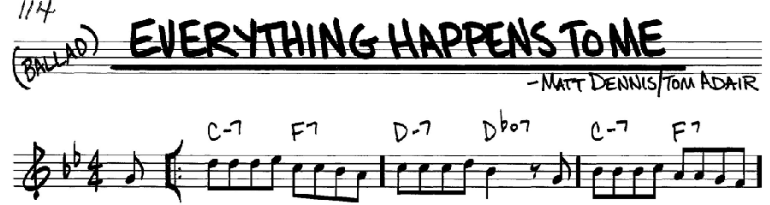
\includegraphics[width=0.5\linewidth]{everything}}. In order to formally solve this problem we need the following proposition.
\begin{proposition}
	Let $K$ be a $\Sigma$-finite kernel (the most general property we can think of) from $(E,\E)$ into $(F,\F)$. We consider measurable functions with respect to the product space: for every positive funtion $f\in\E\otimes\F$ we have that:
	\[Tf(x)=\int_FK(x,\dy)f(x,y)\qquad x\in E\]
	And this object defines a function $Tf\in\E_+$. This is a similar operation to the previous theorem. Moreover the transformation $T:(\E\otimes\F)_+\mapsto \E_+$ is linear and continuous under increasing limits, that is:
	\begin{enumerate}[a)]
		\item if we take $f,g\in(\E\otimes\F)_+$ and $a,b\in\R_+$ we have
		\[T(af+bf)=aTf+bTg;\]
		\item $Tf_n\nearrow Tf$ for $\every$ sequence $(f_n)_{_{n}}\subset(\E\otimes\F)_+$ with $f_n\nearrow f$.
	\end{enumerate}
\end{proposition}
So, similarly to the previous theorem we have constructed this operator $Tf$ which operates on the function set $(\E\otimes\F)_+$ giving us a positive $\E$-measurable function. So we can start from this function to build a method to construct measures on the product space $(\E\otimes\F)_+$ with its related \sa{}.
\begin{theorem}
	\emph{Extension of measures on product spaces}.\\
	Let $\mu$ be a measure on the measurable space $(E,\E)$. Let $K$ be a $\Sigma$-finite\footnote{Erm... what the sigma?} transition kernel from space $(E,\E)$ into $(F,\F)$. Then:
	\begin{enumerate}[\circnum]
		\item if we take our function $f(x,y)$, integrate it against our kernel $K(x,\dx)$ over $F$ and then integrate again against measure $\mu$ over $E$, the operation 
		\[\pi f=\int_E\mu(\dx)\int_FK(x,\dy)f(x,y)\]
		defines a measure $\pi$ on $(E\times F,\E\otimes\F)$;
		\item if $\mu$ is $\sigma$-finite and $K$ is $\sigma$-bounded then $\pi$ is $\sigma$-finite and it is the unique measure on $(E\times F,\E\otimes\F)$ satisfying
		\[\pi(A\times B)=\int_A\mu(\dx)K(x,B)\qquad\every A\in\E,B,\in\F.\]
	\end{enumerate}
\end{theorem}
So by means of kernels we are able to define measures on product spaces in this way\footnote{I crave to be released from this prison of flesh.}.
\begin{remark}
	When the kernel that we used to extend the measure has the form 
	\[K(x,B)=\nu(B)\]
	for some $\Sigma$-finite measure $\nu$ on $(F,\F)$, which means that it only depends on $B$ and is therefore a measure, then we obtain the \emph{product measure}
	\[\pi=\mu\nu.\]
\end{remark}
But what should we do when we have more than 2 spaces\footnote{I have an idea.}? On finite product spaces we introduce in the same manner the product measure 
\[\pi=\mu_1\mu_2\cdots\mu_n\]
where $\mu_i$ is $\Sigma$-finite on $(E_i,\E_i)$ for $\every i=1,\ldots,n$.
So we can induce the presence of another measure from the product measure using the kernels, without assuming independence in the construction.
\begin{example}
	Here we tackle $n=3$. Take $\mu_1$ on $(E_1,\E_1)$, the transition kernel $K_2$ from $(E_1,\E_1)$ into $(E_2,\E_2)$ and the transition kernel $K_3$ from $(E_1\times E_2,\E_1\otimes\E_2)$ into $(E_3,\E_3)$. Not how we only defined the first measure and then only the transition kernels. We will use these fucking kernels to "move" from measure to measure and from space to space. We have
	\[\pi f=\int_{E_1}\mu(\dx_1)\int_{E_2}K_2(x,\dx_2)\int_{E_3}K\Big((x_1,x_2),\dx_3\Big)f(x_1,x_2,x_3)\]
	with $f$ positive and $(\E_1\otimes\E_2\otimes\E_3)$-measurable. So we defined a measure $\pi$ which is different from the product measure we recalled earlier (actually that product measure is a special case of this measure) and $\pi$ is a measure on the 3-dimensional product space. Writing $\pi$ in differential form:
	\begin{align*}
		\pi(\dx_1,\dx_2,\dx_3)&=\mu(\dx_1)K_2(x,\dx_2)K\Big((x_1,x_2),\dx_3\Big)\\
		&=\mu_1K_2K_3.
	\end{align*}
\end{example}
This is for finite product spaces but we can also extend this to infinte product spaces\footnote{Why. Stop.}.\\
What should we expect now?
\section{Expectation}
Well that was a cheap joke. We already know the meaning of expectation from our undergraduate courses... but here we will rock our world and learn some new interpretations. Let's start with measure theory\footnote{We have a great time ahead, I see.}. In probability the concept of expectation is strictly tied with the concept of integral: we could say they are almost the same thing.
\begin{definition}
	Let $X$ be a real valued $(\overline{\R})$ \rv{} on the probability space $(\Omega,\mathscr{H},\pr)$. The \emph{expectation} or \emph{expected value} of $X$ is
	\[\ev X=\int_\Omega X(\omega)\pr(\dw).\]
\end{definition}
	\begin{notation}
		\[\ev X=\int_\Omega X(\omega)\pr(\dw)=\int_\Omega x\dif\pr.\]
		There is always the compact notation we use for integrals
		\[\pr X.\]
	\end{notation}
We are integrating the function over the space where it is defined, but since we are using Lebesgue integration we need to integrate with respect to a measure... which is the probability measure $\pr(\dw)$. This is a little bit different from the classic definition, but this is more correct.
\begin{remark}
	The expectation of $X$ exists \underline{if and only of} the related integral exists. So the existence of the expectation is the existence of the integral.\\
\end{remark}
\begin{wrapfigure}{R}{0.6\textwidth}
	\centering
	
\includegraphics[width=\linewidth]{kept3}
	\caption{And then he turned himself into a pickle, funniest shit I've ever seen.}
	\label{fig:kept3}
\end{wrapfigure}
Consider the \rv{} $X$, with its positive part $X^+$ and its negative part $X^-$. Moreover, remember that 
\[X=X^+-X^-\]
where both the positive part \textit{and} the negative part are positive functions (remember?\footnote{No. Happy?}). If we apply the expectation to $X$, by the linearity of the integral operator we have that:
\[\ev X=\ev X^+-\ev X^-.\]
The problem arises when both the expectation of the positive part and the expectation of the negative part are simultaneously infinite.\\
Further, we say that $\ev X$ exists finit e when at the same time both expectations are finite: 
\[\ev X^+<+\infty,\quad X^-<+\infty.\]
In this case
\[\ev X=\ev X^+-\ev X^-<\infty.\]

\vspace*{1cm}

Finally, remember from undergraduate courses:
\[\ev X^+\ev X^-=\ev |X|\]
So if we check that the expectation of the absolute value is finite this will imply that the expectation of $X$ is finite in both the negative and the positive part. A \rv{} with finite expectations is said to be \emph{integrable}.
\begin{remark}\label{eh}
	This is connected to the definition of expectation of a \rv{} that we already know. Consider the "change of variable" formula for Lebesgue integrals (see \cinlar, formula 5.3 page 30): consider $f\in\E$ and $h:(F,\F)\mapsto(E,\E)$. We integrate
	\[\int_F\nu(\dx)f\Big(h(x)\Big)=\int_E\mu(\dy)f(y)\]
	where $\mu$ is a measure on $(E,\E)$ and is the \textit{image measure} of $\nu$ through the function $h$. For us:
	\begin{itemize}
		\item $h\equiv X$;
		\item $(F,\F)\equiv(\Omega,\mathscr{H})$;
		\item $\nu=\pr$;
		\item $\mu$ is the distribution of $X$;
		\item $(E,\E)\equiv(\R,\B_{\R}$.
	\end{itemize}
	So the formula becomes
	\[\int_\Omega\pr(\dw)f\Big(X(\omega)\Big)=\int_{\R}\mu(\dx)f(x)\]
	with $f$ Borel-measurable. Now the last step is to choose a specific function $f$, for which we choose the \textit{identity function} so that
	\[\int_\Omega\pr(\dw)X(\omega)=\int_{\R}\mu(\dx)x.\]
	Here's the formula that we used to calculate the expectation in the undergraduate years! To be honest, that's what you'll ever really use in the sad case of you working in this field. If the distribution is absolutely continuous with respect to the lebesgue measure we get
	\[\int_{\R}\mu(\dx)x=\int_{\R}f_X(x)\dx\cdot x\]
	otherwise, if it is absolutely continuous with respect to a counting measure we get
	\[\int_{\R}\mu(\dx)x=\sum_{i=1}^{\infty}\pr(X=x_i)\cdot x_i.\]
	\begin{notation}
		Forget riemann integrals and sums, fucker, from now on you must learn to use 
		\[\int_{\R}\mu(\dx)x.\]
	\end{notation}
\end{remark}
\subsection{Properties of expectation}
\begin{itemize}
	\item \emph{Positivity}:
	\[X\geq0\implies\ev X\geq0.\]
	Remember that we are talking about \rv s, so when we say $X\geq 0$ we actually mean ``$X\geq 0$ almost surely with respect to $\pr$''\footnote{Because reality crumbles in front of the chaotic horror of randomness. A similar fate is reserved to my balls.}.
	\item \emph{Monotonicity}:
	\[X\geq Y\geq0\implies\ev X\geq\ev Y.\]
	\item \emph{Linearity}:
	\[X,Y\geq0\implies\ev(aX+bY)=a\ev X+b\ev Y.\]
	\item \emph{Insensitivity}:
	\[X,Y\geq0,\; X=Y\text{ almost surely }\implies\ev X=\ev Y.\]
	\item \emph{Monotone convergence}: if we have, for $X_n\geq-0$,
	\[(X_{n})_{_{n}}\nearrow X\implies\ev X_n\nearrow \ev X.\]
	\item \emph{Fatou's Lemma}: for $X_n\geq0$ we have
	\[(X_{n})_{_{n}}\implies\ev\liminf X_n\leq\liminf\ev X)n.\]
	\item \emph{Dominated convergence}: if $(X_{n})_{_{n}}$ is a sequence of \rv s such that $\every n |X_n|\leq Y$ and $Y$ has finite expectation (it is integrable) and $\lim_{n\to\infty}X_n$ exists, then 
	\[\ev\lim_{n}X_n=\lim_{n}\ev X_n.\]
	\item \emph{Bounded convergence}: if we have a sequence of \rv s $(X_n)_{_{n}}$ such that $|X_n|\leq b<\infty$ and $\lim_{n\to\infty}X_n$ exists, then
	\[\ev\lim_{n}X_n=\lim_{n}\ev X_n.\]
\end{itemize}
\begin{remark}
	$X$ is positive (or non negative) and $\ev X=0$ \underline{if and only if} $X=0$ almost surely. 
\end{remark}
\begin{remark}
	If we restrict $\ev X$ and $\ev Y$ on the subset $H$ we get:
	\[\text{if }\ev X\indi_H\geq\ev Y\indi_H\quad\every H\implies X\geq Y\text{ a.s.}\]
\end{remark}
\begin{theorem}
	Let $X$ be a \rv{} taking values in $(E,\E)$ and be measurable relative to $\mathscr{H}$ and $\E$. If $\mu$ is the distribution of $X$ then
	\begin{equation}
		\ev f\circ X=\mu f,\qquad\every f\in\E_+ \tag{$\star$} \label{diocane}
	\end{equation}
	Conversely, if \ref{diocane} holds for some measure $\mu$ on $(E,\E)$ and $\every f\in\E_+$, then $\mu$ is the distribution of $X$.
\end{theorem}
\begin{fancyproof}
	The proof should be simple. The first statement is basically the \hyperref[eh]{change of variable} formula, rephrasing the theorem on integration with respect to image measures.
	The second converse statement requires more thought. If \ref{diocane} holds $\every f\in\E_+$, then it holds also for $f=\indi_A$ for $A\in\E$ and we have that if we want to calculate the measure 
	\[\mu(A)=\mu\indi_A=\ev\indi_A\circ X=\pr(X\in A).\]
	So we have identified this measure with the distribution of the random variable and hence $\mu$ is the distribution of $X$.
\end{fancyproof}
\begin{example}
	\begin{enumerate}[\circnum]
		\item The \emph{variance} of the \rv{} $X$ is
		\[\var X=\ev(X-\ev X)^2.\]
		\item Consider the expectation of an exponential transform of $X$:
		\[\tilde{\mu}_r=\ev e^{-rX}=\int_{\R_+}e^{-rx}\mu(\dx),\qquad r\in\R_+,x>0.\]
		This is known as the \emph{Lapalce transform} of distribution $\mu$. It is connected to the moment generating function of a distribution.
		\item We could be interested in the expectation of another exponential transform:
		\[\hat{\mu}_r=\ev e^{irX}=\int_{\R}\mu(\dx)e^{irx}\]
		and, exploiting the representation of complex numbers,
		\[\hat{\mu}_r=\int_{\R}\mu(\dx)\cos(rx)+i\int_{\R}\mu(\dx)\sin(rx)\]
		and this is called the \emph{characteristic function} of $\mu$.
		\item Consider $X$, a \rv{} taking values in $\overline{\N}$. Consider
		\[\ev z^X=\sum_{n=1}^{\infty}z^n\cdot\pr(X=n),\qquad z\in[0,1].\]
		This is called \emph{probability generating function of $X$}.
	\end{enumerate}
	These are all special kinds of expectations.
\end{example}
\begin{remark}
	The expectation $\ev X$ is in some sense ``optimal'': what the fuck? It is ``optimal'' because it is our best estimate of $X$. Imagine we are given the following integral:
	\[f(a)=\int_\Omega \Big(X(\omega-a)\Big)^2\pr(\dw).\]
	Let us now derive the minimum value for the number $a$, that is the best value that cancels out the random variable $X$. Just take the derivative with respect to $a$:
	\begin{align*}
		\frac{\dif}{\dif a}f(a)&=\int_\Omega\pr(\dw)\Bigg(-2\Big(X(\omega)-a\Big)\Bigg)=0\\
		&=2a\int_\Omega\pr(\dw)-2\int_\Omega\pr(\dw)X(\omega)=0\\
		&\implies a= \underbracket{\int_\Omega\pr(\dw)X(\omega).}_{\mathclap{\text{definition of }\ev X}}
	\end{align*}
\end{remark}
We must now recall some famous inequalities.
\begin{itemize}
	\item \emph{Markov inequality}: this is for positive, real-valued random variables. Let $X$ be a positive and real-valued \rv. We may be interested in the probability that $X$ exceeds some positive value $b$. We know that
	\[\pr(X>b)\leq\frac{1}{b}\ev X\qquad\every b>0.\]
	\item \emph{Chebyshev inequality}: this is too for positive, real-valued random variables. Let $X$ be a positive and real-valued \rv. What we have is that
	\[\pr\Big(|X-\ev X|>\varepsilon\Big)\leq\frac{\var X}{\varepsilon^2},\qquad\epsilon>0.\]
	\item \emph{Jensen inequality}: Let $X$ be a real-valued \rv{} with finite expectation (integrable) and let $f$ be a convex function on $\R$. Then
	\[\ev f(X)\geq f(\ev X).\]
	If the function is concave the inequality is the opposite.
\end{itemize}
\end{document} 
%THIS IS THE DARK AGE OF LOVE 